\documentclass[11pt]{article}

\usepackage[T1]{fontenc}
\usepackage[utf8]{inputenc}
\usepackage[margin=0.88in]{geometry}
\usepackage{amsmath,amssymb}
\usepackage{graphicx}
\usepackage{booktabs}
\usepackage{array}
\usepackage{longtable}
\usepackage{tabularx}
\usepackage{enumitem}
\usepackage{xcolor}
\usepackage{microtype}
\usepackage[round,authoryear]{natbib}
\usepackage[hidelinks]{hyperref}
\usepackage{url}

\definecolor{deepblue}{HTML}{17365D}
\definecolor{softblue}{HTML}{EAF1F8}
\definecolor{softgray}{HTML}{F3F4F6}
\definecolor{darkgray}{HTML}{343A40}
\hypersetup{colorlinks=true,linkcolor=deepblue,citecolor=deepblue,urlcolor=deepblue}
\urlstyle{same}
\setlist{nosep,leftmargin=1.5em}
\setlength{\parindent}{0pt}
\setlength{\parskip}{0.55em}
\setlength{\tabcolsep}{5pt}
\setlength{\emergencystretch}{2em}
\renewcommand{\arraystretch}{1.14}
\graphicspath{{figures/}}
\newcommand{\R}{\mathbb{R}}
\newcommand{\E}{\mathbb{E}}
\newcommand{\method}[1]{\texttt{#1}}
\newcommand{\resultbox}[1]{%
  \begin{center}\fcolorbox{deepblue}{softblue}{\parbox{0.93\linewidth}{#1}}\end{center}}

\title{\textbf{What We Learned from Conditional Generative Models of NeuroPAL Dynamics}\\[0.35em]
\large From point prediction and diffusion experiments to regularized conditional flow matching}
\author{Internal scientific methods report\\\texttt{new\_sbtg\_neuro}}
\date{1 September 2026}

\begin{document}
\maketitle

\begin{abstract}
This report reconstructs the model-development path for one-step probabilistic forecasting of observed NeuroPAL calcium activity and asks why the selected conditional flow-matching model performed well. It inventories the broader screens of ordinary and Gaussian-source flows, bounded energy-ratio models, denoising-score matching, mixture-density networks, RealNVP, and Gaussian families. The main quantitative evidence comes from a corrected cohort of 17 OH16230 worms, 54 head neurons, five whole-worm outer folds, and a 0.25 s forecast horizon. Older benchmark scores are retained only as development evidence because they used different cohorts, sampling schemes, or evaluation banks. On the corrected benchmark, the flow has a 4.20\% lower multivariate energy score than the strongest matched Student-$t$ competitor, and a 3.73\% lower sample-mean RMSE. However, independently shuffling generated sample identities across neurons, conditional on each history, leaves the flow's energy score essentially unchanged. History-dependent Gaussian variance and Student-$t$ tails each produce small but reproducible marginal improvements. The flow also overpredicts a predeclared large-innovation event. The most defensible interpretation is therefore that the flow succeeds mainly through a strong residual location model plus flexible per-neuron conditional distributions, while useful residual cross-neuron dependence is modest under the tested one-step diagnostics. Flow matching offers a comparatively simple simulation-free regression objective and deterministic ODE sampling, which can aid engineering stability, but the experiments do not establish a general theorem or a universal long-rollout advantage.
\end{abstract}

\tableofcontents
\clearpage

\section{The question and the answer}

The scientific target is the conditional law
\begin{equation}
 p\!\left(x_{t+1}\mid x_{t-L+1:t},s_{t-L+1:t}\right),
 \label{eq:estimand}
\end{equation}
where $x_t\in\R^{54}$ is the observed neural calcium vector, $s_t$ is the aligned binary stimulus indicator, the recording rate is 4 Hz, and the forecast horizon is one frame (0.25 s). This is a forecast distribution for observed activity. It is not a causal graph, a synaptic model, or a decomposition of biological and measurement noise.

\resultbox{\textbf{Main conclusion.} The selected flow is the best tested one-step sampler under the prespecified multivariate energy score, but the new ablations narrow the reason. Its advantage is not primarily explained by residual coupling between neurons. The evidence instead points to accurate conditional location, some history-dependent scale, and distributional flexibility beyond a single elliptical family. This is useful evidence about the predictive structure of the data, but it does not prove multimodality or identify a biological noise mechanism.}

Four findings matter most:
\begin{enumerate}
  \item A deterministic mean alone is insufficient for the question because squared error estimates a conditional mean, not a distribution.
  \item Recent neural and stimulus history carries strong predictive information, but adding more elaborate encoders or forcing the full declared 20 s window into the receptive field did not improve the held-out score.
  \item Once history is known, changing marginal uncertainty and moderately heavy tails help, while remaining joint residual dependence contributes little to the headline energy advantage.
  \item The flow is not uniformly calibrated: it predicts too many large one-step innovations under the prespecified tail event. Model choice must therefore follow the downstream quantity, not a single leaderboard rank.
\end{enumerate}

\section{Data, target, and validation design}

The current comparison uses 17 OH16230 worms imaged with NeuroPAL-style neuronal identities \citep{yemini2021neuropal}, 54 retained head neurons, and recordings sampled at 4 Hz. Each input contains 80 frames (20 s) of neural and binary-stimulus history. The model predicts the residual
\begin{equation}
 \Delta x_{t+1}=x_{t+1}-x_t,
 \qquad x_{t+1}=x_t+\Delta x_{t+1},
 \label{eq:residual}
\end{equation}
rather than predicting the full next state from scratch. Residualization gives the network an explicit persistence baseline and focuses capacity on the smaller innovation.

The split unit is the whole worm. Five fixed outer folds ensure that every reported target comes from an animal excluded from that model's fitting and early stopping data. The current run uses two model seeds and two sampling seeds. Metrics are first averaged over these nuisance repeats and then compared over the 17 worms, which are the inferential units. The paired 95\% intervals are percentile bootstrap intervals over worms; exact sign-flip tests are adjusted across the five declared primary comparisons using Holm's procedure \citep{holm1979multiple}.

An implementation detail changes how the 20 s history should be described. The selected legacy temporal convolutional network (TCN) receives 80 frames, but four kernel-3 blocks with dilations 1, 2, 4, and 8 have a direct receptive field of
\[
 1+2(1+2+4+8)=31\ \text{frames}=7.75\ \text{s}.
\]
Thus the input array is 20 s long, while the selected encoder's final output directly uses only the most recent 7.75 s. A later 127-frame full-history TCN did not improve the confirmation score. This suggests that the most useful information may be recent, or that the smaller encoder regularizes better at this sample size. It does not establish a biological memory cutoff at 7.75 s. TCNs are a standard causal sequence-modeling choice with strong empirical memory properties \citep{bai2018tcn}.

\section{How the approach evolved}

The development path was not one clean, directly comparable tournament. It contained a separate synthetic tangent program, an initial pooled neural benchmark, architecture screens, biological-history tests, regularization tests, rollout tests, and finally the corrected distribution-structure experiment. Table~\ref{tab:history} preserves that distinction.

\begin{longtable}{p{0.18\linewidth}p{0.25\linewidth}p{0.49\linewidth}}
\caption{Model-development evidence. Absolute scores must be compared only within a row because cohorts and evaluation banks changed.}\label{tab:history}\\
\toprule
Stage & Models or question & What was learned \\
\midrule
\endfirsthead
\toprule
Stage & Models or question & What was learned \\
\midrule
\endhead
Synthetic tangent work & Normalized autoregressive Transformer versus legacy diffusion and EDM & On known synthetic laws, both tangent estimators worked for location changes but failed the frozen validity gate for covariance, skew-mixture, and multimodal-occupancy changes. On one 64-dimensional development system, Transformer fair energy was 1.1768, EDM 1.3226, and legacy diffusion 1.7072. Diffusion sampled much faster, but this one-system generation result is directional only. Predictive density or response-score fit did not guarantee a valid derivative with respect to history. \\
\addlinespace
Simple baselines and lag screen & Persistence, multiscale ridge, Gaussian regression & The point-prediction view was useful as a baseline and for selecting history length. In the older pooled 20-worm run, the nested ridge screen selected $L=80$; its energy fell from 1.589 at $L=2$ to 1.466 at $L=80$, non-monotonically. This established that history matters, while showing that a rigid Gaussian baseline leaves predictive structure unused. \\
\addlinespace
First neural density benchmark & TCN Gaussian, two- and four-component mixture-density networks (MDNs), conditional flow & In the older pooled benchmark, flow energy was 1.3948 versus 1.4122 for MDN-4, 1.4249 for the best listed TCN Gaussian, 1.5394 for ridge Gaussian, and 1.6702 for persistence. All five neural finalists were within one reported standard-error band, so the early evidence favored flow without establishing a large architecture separation. MDNs follow the conditional-mixture construction of \citet{bishop1994mdn}. \\
\addlinespace
Broader density tournament & Regularized flows, Gaussian-source flows, bounded energy-ratio models, MDNs, RealNVP, low-rank Gaussian & Two regularized flows led confirmation, 0.8502 and 0.8521 energy, a 0.21\% gap smaller than fold/seed uncertainty. Exact invertible flows such as RealNVP \citep{dinh2017realnvp} and several explicit-density heads did not improve the selected sample score. \\
\addlinespace
History-encoder test & Legacy TCN, full-history TCN, phase TCN, multiscale TCN, GRU, Transformer & The simpler legacy TCN-flow remained best in confirmation (0.8513 versus 0.8541 for full-history TCN and 0.8629 for phase TCN). More nominal context and more expressive sequence encoders were not automatically better. \\
\addlinespace
Regularization test & Dropout, weight decay, history jitter, transition reweighting & A width-128 flow with 15\% dropout and neural-history jitter of 0.01 won confirmation (0.8506 versus 0.8557 for the unregularized control). Its full-cross-validation energy was 1.3895. The small size of several gaps argues for regularization and repeated validation, not a claim that one hyperparameter is uniquely optimal. \\
\addlinespace
Rollout check & Selected flow versus MDN and flow controls, 0.25--10 s & At 0.25 s the selected flow led energy (0.8652 versus 0.8755 for MDN). At 10 s the MDN had slightly better energy (4.4375 versus 4.5056) and balanced energy, while the flow had a better variogram (0.1887 versus 0.2414) and nearly identical RMSE. The best model is horizon- and metric-dependent. \\
\addlinespace
Corrected structure experiment & Flow, fixed/conditional diagonal Gaussian, rank-8 Gaussian, rank-8 Student-$t$, dependence shuffle & On the corrected 17-worm cohort, flow retained a 4.20\% energy advantage over Student-$t$. The shuffle and matched-family tests showed that joint residual dependence explains little of that advantage; changing variance and heavier tails help modestly. \\
\bottomrule
\end{longtable}

The diffusion experiments deserve special care. They were conducted in a separate, known-law synthetic tangent benchmark, not as an apples-to-apples precursor on the corrected 17-worm cohort. Diffusion models learn a sequence of noisy reverse transitions or a score field \citep{ho2020ddpm,song2021sde}. The synthetic study showed a useful general lesson: an apparently good generator or response score can still have a poor derivative with respect to conditioning history. It did not show that diffusion is universally inferior for neural generation.

\subsection{The full density and energy-model screen}

The final corrected-cohort table later in this report is intentionally narrow because that experiment was designed to isolate dependence, changing variance, and elliptical tail shape. It should not be read as the complete model tournament. Table~\ref{tab:fullscreen} restores the full 16-candidate atlas-blind screen. This was the older pooled 20-worm protocol, using selection folds 0--2 and three trials per candidate. It is development evidence, not a direct extension of the corrected 17-worm scoreboard.

{\scriptsize
\begin{longtable}{p{0.34\linewidth}rrrrr}
\caption{Full focused density screen on the older pooled cohort. Lower is better except coverage, whose target is 0.90. The model labels expose the family and principal hyperparameter.}\label{tab:fullscreen}\\
\toprule
Candidate & Energy & Balanced & Variogram & RMSE & Cov. 90 \\
\midrule
\endfirsthead
\toprule
Candidate & Energy & Balanced & Variogram & RMSE & Cov. 90 \\
\midrule
\endhead
CFM, width 128, dropout 0.10 & 1.7370 & 1.7609 & 0.05767 & 0.33664 & 0.8339 \\
CFM, width 64, dropout 0.10, WD $10^{-3}$ & 1.7413 & 1.7628 & 0.05831 & 0.33741 & 0.8444 \\
CFM, compact width 48 & 1.7466 & 1.7641 & 0.05947 & 0.33888 & 0.8555 \\
CFM, unregularized control & 1.7559 & 1.7769 & 0.05894 & 0.33996 & 0.8384 \\
MDN, 4 autoregressive components & 1.7868 & 1.8051 & 0.06078 & 0.35329 & 0.7766 \\
MDN, 8 autoregressive components & 1.7914 & 1.8103 & 0.06103 & 0.35478 & 0.7797 \\
Bounded energy ratio, $B=0.5$, base weight 0.25 & 1.8009 & 1.8189 & 0.06177 & 0.35492 & 0.8133 \\
Bounded energy ratio, $B=1.0$, base weight 0.25 & 1.8033 & 1.8196 & 0.06163 & 0.35456 & 0.8129 \\
Bounded energy ratio, $B=1.0$, base weight 0.50 & 1.8030 & 1.8201 & 0.06161 & 0.35454 & 0.8132 \\
Bounded energy ratio, $B=1.5$, base weight 0.50 & 1.8049 & 1.8210 & 0.06152 & 0.35476 & 0.8123 \\
Gaussian-source CFM, base weight 0.10 & 1.8068 & 1.8241 & 0.06159 & 0.35539 & 0.8081 \\
Gaussian-source CFM, base weight 0.25 & 1.8075 & 1.8248 & 0.06162 & 0.35553 & 0.8072 \\
Gaussian-source CFM, base weight 1.00 & 1.8070 & 1.8249 & 0.06204 & 0.35594 & 0.8064 \\
Gaussian-source CFM, base weight 0.50 & 1.8070 & 1.8249 & 0.06205 & 0.35595 & 0.8065 \\
RealNVP, 8 affine coupling layers & 1.8141 & 1.8306 & 0.06343 & 0.35814 & 0.8059 \\
Gaussian, conditional rank 16 & 1.8112 & 1.8311 & 0.06283 & 0.35722 & 0.8261 \\
\bottomrule
\end{longtable}
}

Only four candidates advanced to untouched-fold confirmation: wide CFM (energy 0.8502), regularized width-64 CFM (0.8521), MDN-4 (0.8566), and the best bounded energy-ratio model (0.8624). The first two were a near tie relative to fold/seed variation. The consistent screen ordering is still informative: all four Gaussian-source CFM models, all four bounded energy-ratio models, RealNVP, and the rank-16 Gaussian scored below the ordinary CFM variants. But the unconfirmed rows remain screening results and should not be promoted to final biological evidence.

The phrase \emph{energy model} also needs disambiguation. The bounded energy-ratio head was not trained by directly minimizing the evaluation energy score. It learned
\begin{equation}
 p_\theta(y\mid h)\ \propto\ q_\theta(y\mid h)
 \exp\!\left[B\tanh f_\theta(y,h)\right],
 \label{eq:energytilt}
\end{equation}
where $q_\theta$ is a learned diagonal Gaussian reference. A data-versus-reference classifier estimates the bounded density tilt, with Gaussian NLL regularizing the reference, and exact samples use rejection sampling. This is related to density-ratio or noise-contrastive estimation \citep{gutmann2010nce}; \emph{energy score} is the separate held-out metric in Equation~\ref{eq:energy}.

\subsection{The separate denoising-score objective screen}

A later higher-order neural screen added a constrained Gaussian denoising-score-matching (DSM) head. DSM learns a response score from noise-corrupted targets \citep{hyvarinen2005score,vincent2011denoising}, but this comparator remained a Gaussian location-scale family; changing the objective did not give it a non-Gaussian sampler. Table~\ref{tab:scorescreen} reports the complete current-54 selection screen. It used the older 20-worm current cohort and a 32-frame history. Models with three trials covered screen folds 0--2; four one-trial rows were preliminary fold-0 screens and carry substantially weaker evidence.

\begin{table}[ht]
\centering
\scriptsize
\caption{Higher-order objective screen on the older 20-worm current-54 cohort. The trial count is essential: one-trial rows were not replicated across screen folds.}
\label{tab:scorescreen}
\begin{tabular}{lrrrrr}
\toprule
Candidate & Energy & Balanced & Variogram & RMSE & Trials \\
\midrule
Wide CFM & 1.7450 & 1.8056 & 0.05769 & 0.33690 & 3 \\
MDN-4 & 1.7906 & 1.8419 & 0.05991 & 0.35110 & 3 \\
Bounded energy ratio & 1.8065 & 1.8549 & 0.06096 & 0.35311 & 3 \\
Rank-4 Gaussian & 1.8101 & 1.8611 & 0.06118 & 0.35367 & 3 \\
Gaussian-source CFM & 1.8228 & 1.8405 & 0.06286 & 0.35837 & 1 \\
Diagonal heteroskedastic Gaussian & 1.8294 & 1.8547 & 0.06186 & 0.35673 & 1 \\
Constrained Gaussian DSM & 1.8300 & 1.8517 & 0.06209 & 0.35789 & 1 \\
Rank-8 Gaussian & 1.8379 & 1.8562 & 0.06394 & 0.36211 & 1 \\
\bottomrule
\end{tabular}
\end{table}

The DSM head did not advance to confirmation. MDN-4, wide CFM, and the rank-4 Gaussian did; MDN-4 narrowly led confirmation energy (0.8752 versus 0.8778 for CFM), reinforcing that the architecture ranking varies with fold subset, history length, and protocol. The score-based objective therefore supplied a useful negative control, but not evidence that score matching is intrinsically poor.

\section{The selected conditional flow model}

Let $h$ be the TCN encoding of the observed history and $y=\Delta x_{t+1}$ the standardized residual target. Training draws independent $z\sim\mathcal N(0,I)$ and $\tau\sim\mathrm{Uniform}(0,1)$, forms the straight interpolation
\begin{equation}
 x_\tau=(1-\tau)z+\tau y,
\end{equation}
and minimizes
\begin{equation}
 \mathcal L_{\mathrm{FM}}(\theta)
 =\E_{h,y,z,\tau}\left[
 \left\|v_\theta(x_\tau,h,\tau)-(y-z)\right\|_2^2
 \right].
 \label{eq:fm}
\end{equation}
This is conditional flow matching: a network regresses the velocity field of prescribed probability paths without integrating an ODE inside the training loop \citep{lipman2023flow,tong2024otcfm}. At inference, samples start from Gaussian noise and solve
\begin{equation}
 \frac{d x_\tau}{d\tau}=v_\theta(x_\tau,h,\tau),\qquad \tau:0\rightarrow1.
\end{equation}
The implementation uses a deterministic 24-step Heun solver once the base noise and seed are fixed. Its flow head has hidden width 128 and four layers. The history encoder has width 128; optimization uses AdamW at learning rate $3\times10^{-4}$, weight decay $7.5\times10^{-4}$, 15\% dropout, gradient clipping, early stopping, and one copy with 0.01 Gaussian jitter added only to neural history. AdamW decouples weight decay from the adaptive gradient update \citep{loshchilov2019adamw}; dropout is a standard ensemble-like regularizer \citep{srivastava2014dropout}. Small-noise training can act as a local smoothness regularizer under classical differentiability assumptions \citep{bishop1995noise}, but that theorem is motivation rather than a guarantee for this network.

The learned transport can represent distributions that are skewed, non-elliptical, or multimodal without fixing a mixture count. Unlike a Gaussian or Student-$t$ head, it does not expose a closed-form normalized likelihood. Unlike the RealNVP family tested here, its training objective does not require an exactly invertible architecture with a tractable Jacobian. Unlike conventional diffusion training, the selected method uses a single continuous transport field and a short deterministic ODE solve. These are design properties, not explanations by themselves; the held-out ablations determine which properties mattered in these data.

\section{Alternatives and what each tests}

\textbf{RMSE or Gaussian point prediction.} Squared error is minimized by the conditional mean. It answers ``what is the expected next vector?'' but cannot distinguish two predictive laws with the same mean and different variance, tails, or dependence. RMSE remains useful for checking the location component of any generator.

\textbf{Fixed and history-dependent diagonal Gaussian.} These impose independent normal residuals. Holding the fitted mean exactly fixed while changing only fixed versus conditional standard deviations isolates predictable heteroskedasticity around that mean.

\textbf{Rank-8 Gaussian.} A diagonal plus rank-8 covariance term allows history-dependent cross-neuron covariance while retaining an elliptical, light-tailed law. Rank 8 is a modeling choice, not an inferred biological latent dimension.

\textbf{Rank-8 Student-$t$.} This keeps the same covariance parameterization and adds a fitted global degrees-of-freedom parameter, allowing heavier elliptical tails and outlier robustness \citep{lange1989student}. Because the entire model is refit under its own likelihood, the real-data difference is not a pure tail-shape intervention.

\textbf{Gaussian-source flow.} This model first learns a history-dependent diagonal Gaussian mean and scale, then transports samples from that conditional Gaussian toward the target. Its loss combines Gaussian NLL with flow regression. It asks whether the flow benefits from having location and scale solved explicitly before learning non-Gaussian corrections. All tested versions underperformed ordinary Gaussian-base CFM in the broad screen. That may reflect optimization or capacity allocation; it does not prove that conditional scale is irrelevant.

\textbf{Bounded energy-ratio model.} This model tilts a learned Gaussian reference by the bounded energy in Equation~\ref{eq:energytilt}. The bound makes the normalizer finite and rejection sampling possible. It can learn non-Gaussian shape without an invertible map, but the bounded tilt and Gaussian proposal restrict how far it can move mass. It was the best explicit energy-family candidate and reached confirmation, where it remained competitive but behind CFM and MDN.

\textbf{Denoising-score Gaussian.} The constrained DSM head fits the score of Gaussian-corrupted targets over several noise levels. It controls for training objective while leaving the output family Gaussian. Its screen result was almost identical to the Gaussian NLL head, but each had only one preliminary trial in that screen; no strong objective-level conclusion follows.

\textbf{Mixture-density network.} An MDN can model multimodality explicitly, but requires choosing a component count and can have optimization or component-use issues. MDN-4 was consistently competitive and became better on long-horizon energy in the rollout test.

\textbf{Exact normalizing flow.} RealNVP offers exact density evaluation through an invertible transformation \citep{dinh2017realnvp}; it did not win the internal screen. Exact likelihood was therefore not worth the architectural constraint under the chosen sample-score objective.

\textbf{Diffusion/score model.} Diffusion is flexible and parallel across output coordinates, but usually needs many noise levels or reverse steps. It was useful in the separate synthetic tangent program as a fast high-dimensional sampler, yet did not show a quality advantage there. Conditional flow matching can be viewed as part of the same broad transport family; flow-matching paths can include diffusion paths \citep{lipman2023flow}.

\section{What the metrics mean}

No single scalar verifies a multivariate predictive distribution. Proper scoring rules are constructed so that, in expectation, the true distribution minimizes the score \citep{gneiting2007proper}. We therefore use complementary metrics.

For an observation $y\in\R^d$ and $M$ generated samples $X^{(1)},\dots,X^{(M)}$, the fair finite-ensemble energy estimator is
\begin{equation}
 \widehat{\mathrm{ES}}
 =\frac{1}{M}\sum_{m=1}^{M}\|X^{(m)}-y\|_2
 -\frac{1}{2M(M-1)}\sum_{m\ne m'}\|X^{(m)}-X^{(m')}\|_2.
 \label{eq:energy}
\end{equation}
Lower is better. The first term rewards proximity to the observation; the second rewards appropriate ensemble spread. Energy is a proper multivariate generalization of CRPS, but can have limited sensitivity to incorrect correlation \citep{gneiting2007proper,scheuerer2015variogram}.

Marginal CRPS applies the one-dimensional analogue to each neuron and averages. It tests every neuron's predictive marginal while deliberately ignoring which cross-neuron values appear together in the same generated vector. This makes it ideal for verifying that the dependence shuffle leaves marginals unchanged.

The order-$p$ variogram score, here with $p=0.5$, compares observed and predicted pairwise differences,
\begin{equation}
 \mathrm{VS}_{p}
 =\sum_{i<j}w_{ij}
 \left(
 |y_i-y_j|^p-\E_F|X_i-X_j|^p
 \right)^2.
 \label{eq:variogram}
\end{equation}
It is more sensitive to dependence errors than energy in many settings \citep{scheuerer2015variogram}. The implementation uses all neuron pairs and a finite-ensemble bias correction. An innovation variogram applies the same idea to changes relative to the current state; it is a useful secondary diagnostic because the shared level of calcium activity can dominate next-state differences.

RMSE is computed from the sample mean, $\hat\mu(h)=M^{-1}\sum_m X^{(m)}$, and therefore evaluates point-location accuracy only. Marginal 90\% coverage is the fraction of targets inside predicted 5th--95th percentile intervals. Coverage near 0.90 is meaningful only beside interval width (sharpness): arbitrarily wide intervals can attain high coverage. Exact negative log-likelihood (NLL) is available for Gaussian, Student-$t$, and MDN families, but not for the implemented flow; inventing a flow NLL would be invalid.

For the tail event $A=\{|x_{t+1,j}-x_{t,j}|>2\sigma^{\mathrm{train}}_{\Delta,j}\}$, the Brier score is
\begin{equation}
 \mathrm{BS}=\frac{1}{N}\sum_{n=1}^{N}(p_n-\mathbf 1\{A_n\})^2,
\end{equation}
a proper score for binary probabilities \citep{brier1950verification}. Finally, stimulus-balanced energy weights off, onset, offset, and mixed history strata equally so that common no-stimulus windows cannot dominate model selection.

\section{The two diagnostic experiments}

\subsection{Marginal uncertainty versus joint dependence}

For every conditioning history, generated sample indices are permuted independently for each neuron. If sample $m$ originally contains $(X^{(m)}_1,\ldots,X^{(m)}_{54})$, the shuffled vector contains $(X^{(\pi_1(m))}_1,\ldots,X^{(\pi_{54}(m))}_{54})$ with independent permutations $\pi_j$. This exactly preserves each neuron's empirical predictive distribution, sample mean, interval, and tail probability. It destroys which neuron values co-occur, approximating a product of empirical marginals at finite $M$.

The primary bank uses 128 samples and eight shuffles per history. A 256-particle sensitivity bank checks whether the result is a finite-sample artifact. Marginal CRPS is invariant to numerical precision, as required. A common permutation of entire 54-neuron vectors provides an additional exact joint-score control.

This is a diagnostic intervention on generated samples, not an additive information decomposition. A small score change can mean weak useful dependence, a generator that failed to learn it, or a score with low sensitivity to it. That is why energy, ordinary variogram, and innovation variogram are all reported.

\subsection{Changing variance versus richer distribution shape}

Four matched explicit families use the same residual formulation, TCN architecture, head width/depth, regularization settings, optimizer, fold protocol, and epoch ceiling as the flow: fixed diagonal Gaussian variance, conditional diagonal Gaussian variance, rank-8 conditional Gaussian covariance, and rank-8 Student-$t$. The fixed-variance Gaussian reuses the conditional diagonal Gaussian's fitted mean exactly, so its contrast isolates changing scale around that mean.

The rank-8 Gaussian and Student-$t$ share the same mean and covariance parameterization and shared-parameter initialization; Student-$t$ adds one global tail parameter constrained to $(2.1,50)$. But their weights are independently fitted and their native objectives differ. Consequently, the Student-$t$ contrast is a matched-family comparison, not a perfectly isolated tail-only experiment. Thirty new fits were completed and ten frozen flow checkpoints reused byte-for-byte.

\section{Current corrected-cohort results}

\begin{table}[ht]
\centering
\small
\caption{Corrected 17-worm scoreboard. Lower is better except that coverage should be near 0.90 and interpreted with interval width. Equal worm weights are used.}
\label{tab:scoreboard}
\begin{tabular}{lrrrrrr}
\toprule
Model & Energy & CRPS & Variogram & RMSE & Cov. 90 & Width 90 \\
\midrule
Flow & \textbf{1.02146} & \textbf{0.09971} & \textbf{0.02813} & \textbf{0.19456} & 0.9048 & 0.5938 \\
Flow, neuron-shuffled & 1.02113 & \textbf{0.09971} & 0.02814 & \textbf{0.19456} & 0.9048 & 0.5938 \\
Gaussian, diagonal & 1.06789 & 0.10083 & 0.02956 & 0.20247 & 0.8893 & 0.5918 \\
Gaussian, fixed variance & 1.06894 & 0.10108 & 0.02961 & 0.20250 & 0.8958 & 0.6046 \\
Gaussian, rank 8 & 1.06717 & 0.10094 & 0.02951 & 0.20221 & 0.8996 & 0.6130 \\
Student-$t$, rank 8 & 1.06621 & 0.10044 & 0.02960 & 0.20210 & 0.9094 & 0.6427 \\
\bottomrule
\end{tabular}
\end{table}

\begin{figure}[ht]
\centering
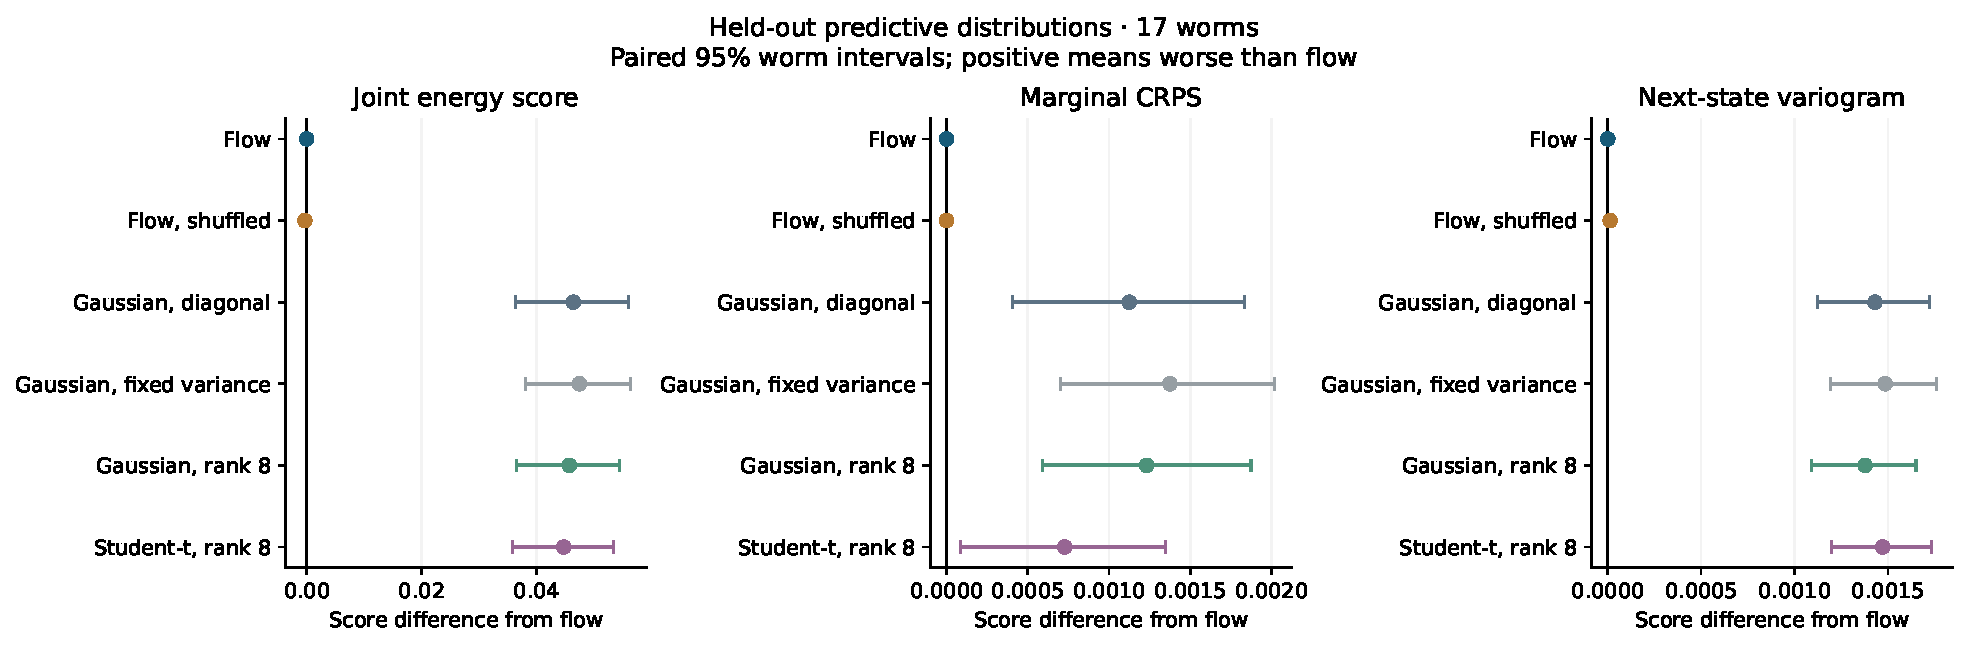
\includegraphics[width=0.96\linewidth]{current_model_comparison.pdf}
\caption{Current model comparison. The plot is generated from held-out predictions on the corrected cohort. Absolute values differ from older leaderboards because the data and evaluation bank changed.}
\label{fig:modelcomparison}
\end{figure}

The five declared primary comparisons are in Table~\ref{tab:paired}. A positive control-minus-candidate difference favors the candidate. The flow improves energy over Student-$t$ by 0.04475, or 4.20\%, in all 17 worms. The flow sample mean also reduces RMSE by 3.73\% relative to Student-$t$ (secondary summary). Changing Gaussian variance improves marginal CRPS by 0.248\%, and Student-$t$ improves marginal CRPS over the matched rank-8 Gaussian by 0.500\%.

\begin{table}[ht]
\centering
\small
\caption{Declared primary paired comparisons. Intervals are worm-level percentile intervals; $p$ values are exact sign-flip tests with Holm adjustment across five tests.}
\label{tab:paired}
\begin{tabularx}{\linewidth}{Xrrrl}
\toprule
Question and metric & Difference & Percent & Positive worms & Holm $p$ \\
\midrule
Keep flow samples joint: energy & $-0.000323$ & $-0.032\%$ & 6/17 & 0.2455 \\
Keep flow samples joint: variogram & $+0.0000127$ & $+0.045\%$ & 13/17 & 0.1171 \\
Conditional vs. fixed Gaussian variance: CRPS & $+0.000251$ & $+0.248\%$ & 13/17 & 0.0320 \\
Student-$t$ vs. rank-8 Gaussian: CRPS & $+0.000505$ & $+0.500\%$ & 13/17 & 0.0201 \\
Flow vs. Student-$t$: energy & $+0.044751$ & $+4.197\%$ & 17/17 & $7.63\times10^{-5}$ \\
\bottomrule
\end{tabularx}
\end{table}

The energy difference after shuffling is $-0.032\%$. Its worm interval runs from $-0.081\%$ to $+0.015\%$. In other words, shuffling does not remove the flow's advantage: the rank-8 Gaussian's gap to flow is 0.04571 before shuffling and 0.04603 afterward. Ordinary variogram evidence also does not pass the adjusted primary test. The secondary innovation variogram does favor intact joint samples by 0.62\%, in 16/17 worms, and the effect repeats at 128 and 256 particles. There is detectable residual joint structure under that diagnostic, but it is small relative to the flow's headline advantage.

\begin{figure}[ht]
\centering
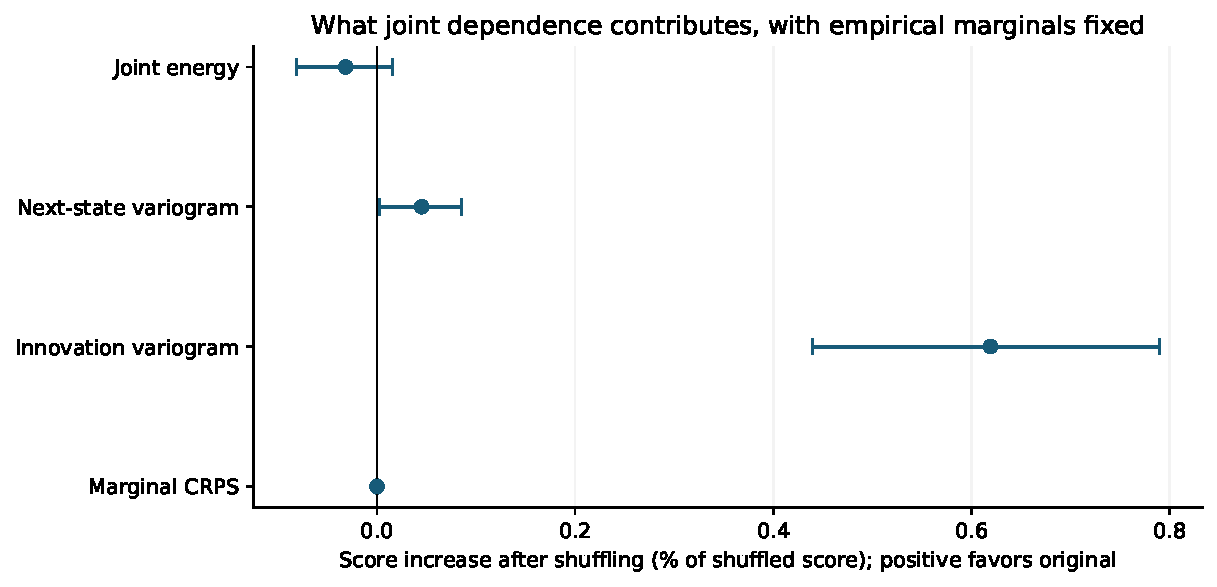
\includegraphics[width=0.94\linewidth]{dependence_ablation.pdf}
\caption{Dependence ablation. Shuffling preserves all empirical marginal distributions and changes only cross-neuron pairing within a conditioning history.}
\label{fig:dependence}
\end{figure}

\subsection{The tail-calibration warning}

The observed large-innovation frequency is 5.91\%. The flow predicts 10.38\%, the rank-8 Gaussian 5.54\%, and Student-$t$ 6.78\%. Tail Brier scores are 0.06411, 0.05570, and 0.05531, respectively. The post-review Student-$t$ versus flow contrast favors Student-$t$ on all 17 worms, but it is exploratory because tail Brier was secondary and this pairwise contrast was not among the five primary tests.

The fitted Student-$t$ degrees of freedom range only from 7.854 to 7.927 after initialization at 8. This supports the practical usefulness of a moderately heavy-tailed family, but it is not a precise empirical estimate of a biological tail index. More broadly, winning average energy does not validate rare-event probabilities. Any tail-based biological analysis should use a separately calibrated model or calibration layer.

\section{What variability the models are learning, and why flow worked well}

The word \emph{variability} covers several different phenomena. Let $H$ denote the observed neural and stimulus history and let $Y=\Delta x_{t+1}$. A location-covariance description writes
\begin{equation}
 Y=\mu(H)+\varepsilon_H,\qquad
 \E(\varepsilon_H\mid H)=0,\qquad
 \operatorname{Cov}(\varepsilon_H\mid H)=\Sigma(H).
 \label{eq:varianceparts}
\end{equation}
Across the population of histories, the law of total variance gives
\begin{equation}
 \operatorname{Var}(Y)
 =\operatorname{Var}_{H}\!\left[\mu(H)\right]
 +\E_H\!\left[\Sigma(H)\right].
 \label{eq:totalvariance}
\end{equation}
The first term is variation in the predictable next-step center as history changes. The second is average uncertainty remaining among outcomes compatible with a history. A fully generative model can additionally change the shape, tails, modes, and dependence of $\varepsilon_H$ with $H$; those properties are not summarized by variance alone.

There is generally only one realized next frame for an exact continuous history. The conditional law is therefore estimated by sharing information across nearby histories, times, and training worms. ``Residual uncertainty'' cannot be equated with intrinsic neuronal randomness. It can contain fluorescence measurement noise, calcium filtering, unobserved behavior or global state, worm-specific effects, imperfect stimulus representation, omitted longer history, and model error, alongside any biological stochasticity. The compared models do not contain a separate latent variable that identifies these sources.

\begin{table}[ht]
\centering
\scriptsize
\caption{Which component of variability each comparison probes. The rows are conceptual components, not an additive numerical decomposition of the flow's score.}
\label{tab:variability}
\begin{tabularx}{\linewidth}{p{0.19\linewidth}p{0.25\linewidth}X}
\toprule
Variability component & Main diagnostic & Evidence and interpretation \\
\midrule
Center across histories, $\mu(H)$ & Sample-mean RMSE; lag and encoder screens & Flow RMSE is 3.73\% lower than Student-$t$. History length and the causal TCN materially improve prediction. A large share of model performance is therefore predictable trajectory, not random spread. \\
Conditional marginal scale & Fixed versus history-dependent diagonal Gaussian with the same fitted mean & Conditional scale improves CRPS by 0.248\%. Uncertainty changes with context, but the effect is modest. \\
Tail/radial shape & Rank-8 Student-$t$ versus rank-8 Gaussian & Student-$t$ improves CRPS by 0.500\% and NLL by 0.0916 nats/neuron. Moderately heavy-tail robustness helps, but fitted degrees of freedom stayed near initialization. \\
Residual cross-neuron dependence & Independent neuron-wise sample-index shuffle within each history & Energy changes by $-0.032\%$ and the primary variogram test does not pass Holm correction. The secondary innovation variogram improves by 0.62\% with intact samples. Some dependence remains, but it is not the main energy advantage. \\
Non-elliptical marginal shape & Flow versus Student-$t$ and Gaussian; marginal CRPS & Flow improves CRPS over Student-$t$ by 0.724\% (secondary) and can represent shape beyond an ellipse. Independent fitted means and encoders prevent assigning this gain to shape alone. \\
Distinct conditional regimes or modes & MDN-2/4/8 and flow screens & MDNs were competitive, and MDN led one higher-order confirmation and 10 s rollout energy, but did not consistently win one-step selection. The data do not provide clear evidence for strong, stable multimodality. \\
Between-worm heterogeneity & Whole-worm folds versus repeated model seeds & Fold variation exceeded seed variation in the early benchmark. Generalization differs more across held-out animals than across optimizer initializations, indicating population heterogeneity or recording differences that the model must absorb. \\
\bottomrule
\end{tabularx}
\end{table}

The experiments support a layered explanation for the flow rather than one dramatic property.

\textbf{Most of the task is conditional location.} Residualization makes persistence explicit, and the TCN extracts recent trajectory and stimulus information. The flow's 4.20\% energy advantage over Student-$t$ is accompanied by a 3.73\% sample-mean RMSE advantage, while marginal CRPS improves by only 0.724\%. These percentages are not additive because the scores use different geometry, but together they make a better conditional center or representation a leading explanation.

\textbf{History-dependent scale and tails matter, but only modestly.} The fixed-variance and Student-$t$ contrasts show real gains of 0.248\% and 0.500\% in marginal CRPS. These effects establish that a constant Gaussian residual is too simple. They do not account cleanly for the entire flow lead, because the contrasts are not additive and the Student-$t$ and flow fit their own encoders and means.

\textbf{Joint residual coupling is not the main explanation.} Shuffling neuron identities within each sample bank preserves every marginal, mean, and interval yet retains the whole energy advantage over the correlated Gaussian. Strong raw neural co-activity can still be present: common past activity, stimulus, and the current level can explain shared movement before the remaining residual is evaluated. The small, stable innovation-variogram effect is evidence against declaring the residuals completely independent.

\textbf{Flexible shape probably helps, but its form remains unidentified.} A flow can learn skewness, context-dependent tails, and multiple local modes. The ordinary CFM variants also beat Gaussian-source CFM, bounded Gaussian energy tilts, RealNVP, and low-rank Gaussian models throughout the broad screen. This suggests that end-to-end transport from a simple source was easier to fit under this sample-size and regularization regime than staged Gaussian correction or tightly constrained transformations. It does not reveal which higher moment the flow used.

\textbf{The tail warning prevents a simple ``better uncertainty'' story.} The flow predicts the large-innovation event almost twice as often as observed and loses tail Brier to Student-$t$. It may obtain a good average energy score by combining a more accurate center with useful broad sample spread while still allocating too much probability to a particular extreme event. The learned uncertainty is useful on average, not uniformly calibrated.

\textbf{The simpler temporal inductive bias and moderate regularization fit this data regime.} Full-history TCNs, phase features, GRUs, Transformers, and multiscale encoders did not beat the legacy TCN in matched confirmation. Dropout, decoupled weight decay, and small neural-history jitter did help. This is compatible with recent dynamics carrying most usable signal and extra capacity overfitting a small number of worms. It remains possible that the screens did not find the best complex model.

The strongest data-level implication is a conditional-residual statement: recent observed history explains much of next-step location and common motion; the remaining forecast distribution has modest history-dependent scale and non-Gaussian shape, a small useful joint component under the innovation variogram, and substantial unresolved variation whose biological and observational sources cannot be separated by these data alone.

\section{Does flow matching have a stability advantage?}

There is a reasonable engineering argument, but it must be divided into optimization, numerical sampling, replication, and rollout stability.

\begin{table}[ht]
\centering
\small
\caption{What can and cannot be said about stability.}
\label{tab:stability}
\begin{tabularx}{\linewidth}{p{0.18\linewidth}X X}
\toprule
Sense of stability & Supporting argument or evidence & Limit \\
\midrule
Training optimization & Equation~\ref{eq:fm} is ordinary stochastic vector-field regression. It does not backpropagate through an ODE solve, and the implementation fixes validation randomness, clips gradients, uses early stopping, and regularizes the encoder. Flow matching was introduced as simulation-free CNF training; published work reports robust/stable training relative to diffusion-path alternatives \citep{lipman2023flow}. & This does not guarantee convex optimization or freedom from seed/fold effects. Fold heterogeneity exceeded seed variation in the early benchmark. \\
Sampling numerics & Given base noise, a deterministic 24-step Heun solve transports the whole 54-vector jointly. Straight conditional training paths are simple targets; related rectified-flow work argues that straighter paths can reduce discretization burden \citep{liu2023rectified}. & The learned velocity field need not yield a globally straight trajectory. We did not prove solver convergence or compare a dense grid of step counts in this experiment. \\
Empirical reproducibility & The selected regularized flow repeatedly led one-step energy across whole-worm folds and seeds. All ten frozen checkpoints replay saved scores exactly; the 128/256-particle dependence result is consistent. & Repeated model and sampling seeds are nuisance checks, not new biological replicates. The same 17 animals were used during development. \\
Free-running rollout & The tested flow produced no $|z|>10$ events through 10 s in the frozen rollout table, and its 10 s RMSE was essentially tied with MDN while its variogram was better. & MDN had better 10 s energy and balanced energy. Absence of an explosion is a necessary numerical check, not evidence of calibrated long-term dynamics. \\
Distributional calibration & One-step coverage was near 0.90 and average energy was best. & The flow overpredicted large innovations and had worse tail Brier than Student-$t$. Stability of generation does not imply calibration. \\
\bottomrule
\end{tabularx}
\end{table}

Flow matching inherits the continuous normalizing flow viewpoint of neural ODEs \citep{chen2018neuralode}. Its main practical simplification is that the expensive differential equation is solved only for sampling, not for every training loss evaluation. This can make training less sensitive to ODE solver tolerances and adjoint errors than maximum-likelihood CNF training. The broad literature also motivates straight or optimal-transport-like paths for faster and more stable simulation \citep{liu2023rectified,tong2024otcfm}. However, the current implementation uses independent Gaussian-to-data pairings rather than minibatch optimal-transport couplings, so claims specific to OT-CFM do not directly apply.

The repository supplies empirical support for repeatability and non-explosive tested rollouts, but not a universal stability theorem. A precise statement is: \emph{the chosen conditional flow combines a simple regression-style training loss with deterministic short-step sampling, and it was reproducible under the seeds, folds, and horizons tested; its long-horizon energy and tail calibration still have important limitations.}

\section{What the data do and do not imply}

\subsection*{Supported interpretations}
\begin{itemize}
  \item Recent trajectory and stimulus history explain a large portion of next-frame location and shared movement.
  \item Residual uncertainty is mildly heteroskedastic: its scale changes predictably with history.
  \item Moderately heavy-tailed robustness helps marginal prediction relative to a matched Gaussian.
  \item Some joint residual dependence remains, most clearly in the innovation variogram, but it contributes little to the selected energy-score advantage.
  \item A flexible conditional sampler improves average one-step prediction beyond the tested elliptical families.
  \item Held-out-animal variation exceeds optimizer-seed variation in the early benchmark, so animal and recording heterogeneity are a material part of the generalization problem.
\end{itemize}

\subsection*{Unsupported interpretations}
\begin{itemize}
  \item Neurons are independent. The result concerns residual predictive dependence after conditioning, not raw neural correlation.
  \item The flow discovered multimodality, a true latent dimension, or a biological noise source. None was isolated.
  \item Residual spread is purely biological stochasticity. Measurement noise, calcium dynamics, omitted state, between-worm differences, and model error remain mixed together.
  \item Rank 8 is a biological dimension, or fitted Student-$t$ degrees of freedom are a biological tail index.
  \item A one-step predictive model identifies anatomy, direct synapses, receptor action, or causal interventions.
  \item The flow is the best model at every horizon or for every decision. MDN led long-horizon energy, and Student-$t$ led the tail-event check.
  \item The synthetic diffusion tangent result is a direct comparison on the final neural cohort.
\end{itemize}

\section{Validation, limitations, and recommended use}

All 30 new explicit-density fits completed; the ten original flow checkpoints were unchanged. Evaluation produced 80 primary archives and 20 particle-sensitivity archives. Forty checkpoints reproduced their saved scores exactly. Thirty fitted densities agreed with independent dense SciPy calculations to a maximum discrepancy of $1.86\times10^{-5}$. Four known-law controls passed, and 289 regression tests passed.

The known-law controls include independent Gaussian, correlated Gaussian, history-dependent Gaussian variance, and covariance-matched Student-$t$ tails. They verify that the shuffle preserves marginals, detects a known joint effect when one exists, and that the scale and tail comparisons can recover their intended signal. They validate the diagnostics, not the biological interpretation.

The principal limitations are repeated use of the same 17 animals during development, overlapping training sets across cross-validation folds, family-specific objectives and stopping behavior, only one fixed rank for the correlated explicit heads, finite sample banks, and a single one-step target for the main conclusion. Flow fits selected epochs 45--49 and stopped at epoch 49, whereas explicit-density alternatives generally selected and stopped earlier. Equal epoch ceilings therefore do not mean equal optimization difficulty or compute.

For one-step sample-based prediction of typical outcomes, the selected flow remains the best-supported choice. For tail probabilities, use the Student-$t$ model or recalibrate and revalidate the flow against tail-specific criteria. For 10 s free-running forecasts, retain MDN as a serious alternative and choose according to the downstream metric. For mechanistic derivatives with respect to history, neither good density score nor good samples are sufficient: the synthetic study shows that the derivative itself needs a known-law calibration gate.

\appendix
\section{Reproducibility map}

The numerical sources used in this report are:
\begin{itemize}
  \item \path{results/distribution_structure_20260831/INSIGHTS.md}
  \item \path{results/distribution_structure_20260831/analysis/REPORT.md}
  \item \path{results/distribution_structure_20260831/analysis/model_scoreboard.csv}
  \item \path{results/distribution_structure_20260831/analysis/paired_comparisons.csv}
  \item \path{results/distribution_structure_20260831/analysis/training_diagnostics.csv}
  \item \path{results/distribution_structure_20260831/VALIDATION.json}
  \item \path{results/conditional_distribution_benchmark/}\newline
        \path{final_overnight_20260826/RESULTS_SUMMARY.md}
  \item \path{results/conditional_distribution_benchmark/}\newline
        \path{atlas_blind_world_model_20260827/REPORT.md}
  \item \path{results/conditional_distribution_benchmark/}\newline
        \path{atlas_blind_world_model_20260827/leaderboard.csv}
  \item \path{results/conditional_distribution_benchmark/}\newline
        \path{biological_world_model_20260828/REPORT.md}
  \item \path{results/conditional_distribution_benchmark/}\newline
        \path{rollout_stability_world_model_v2_20260828/REPORT.md}
  \item \path{results/conditional_distribution_benchmark/}\newline
        \path{rollout_stability_world_model_v2_20260828/rollout_confirmation/REPORT.md}
  \item \path{history_tangent_benchmark/DIFFUSION_VS_AR_SCIENTIFIC_REPORT.md}
  \item \path{results/higher_order_neural_20260828/current54/screen_leaderboard.csv}
  \item \path{results/higher_order_dynamics_20260828/FINAL_REPORT.md}
\end{itemize}

The corrected structure experiment can be regenerated with the repository's \path{conditional_neural_benchmark.distribution_structure_*} runners. Its final validation file records source and checkpoint hashes. The compiled report is documentary and does not alter any frozen benchmark artifact.

\section{A compact decision guide}

\begin{tabularx}{\linewidth}{p{0.27\linewidth}X}
\toprule
Use case & Recommended interpretation or model \\
\midrule
One-step typical predictive samples & Selected regularized conditional flow; validate with energy, CRPS, variogram, RMSE, and coverage. \\
Marginal tail probabilities & Student-$t$ is currently better calibrated for the declared large-innovation event; do not rely on flow energy alone. \\
Long free-running paths & Compare flow and MDN at the actual target horizon; MDN led 10 s energy while flow led the 10 s variogram. \\
Exact likelihood & Gaussian, Student-$t$, MDN, or exact flow families; the implemented conditional flow has no exact NLL. \\
Joint residual questions & Use the innovation variogram and direct dependence diagnostics; energy alone is weakly informative. \\
History derivatives or mechanistic tangents & Require a separate synthetic known-law validity gate. Predictive fit is insufficient. \\
\bottomrule
\end{tabularx}

\clearpage
\bibliographystyle{plainnat}
\bibliography{references}

\end{document}
